%CONFIGURACIÓN DEL DOCUMENTO Y HOJA

\documentclass[11pt,letterpaper]{article}
\setlength{\parindent}{0em}                  %DISTANCIA SANGRÍA
\setlength{\parskip}{0.5em}                  %DISTANCIA ENTRE PÁRRAFOS
\textwidth 6.5in
\textheight 9.in
\oddsidemargin 0in
\headheight 0in

%PAQUETES DEL TEMPLATE

\usepackage{fancybox}
\usepackage[utf8]{inputenc}
\usepackage{epsfig,graphicx}
\usepackage{multicol,pst-plot}
\usepackage{pstricks}
\usepackage{amsmath}
\usepackage{amsfonts}
\usepackage{amssymb}
\usepackage{eucal}
\usepackage[left=2cm,right=2cm,top=2cm,bottom=2cm]{geometry}
\usepackage{txfonts}
\usepackage[spanish]{babel}
\usepackage[colorlinks]{hyperref}
\usepackage{cancel}
\usepackage{caption}
\usepackage{float}
\usepackage{upgreek}
\usepackage{gensymb}
\usepackage{subfigure}
\usepackage{siunitx}
\usepackage{color}
\usepackage{tikz}
\usepackage{listings}

\usepackage{mdframed}
\usepackage[
backend=bibtex,
style=ieee,
sorting=none
]{biblatex}
\addbibresource{biblio.bib}
\usepackage{multicol}
\usepackage{stackrel}

%DEFINICIÓN DE COLORES EXTRAS

\definecolor{codegreen}{rgb}{0,0.6,0}
\definecolor{codegray}{rgb}{0.5,0.5,0.5}
\definecolor{backcolour}{rgb}{0.95,0.95,0.95}
\hypersetup{colorlinks=true,linkcolor=codegreen,citecolor=blue,filecolor=blue,urlcolor=magenta,}

%CONFIGURACIÓN DE LSTLISTINGS PARA CÓDIGOS

\lstset{ %
language=python,                % choose the language of the code
basicstyle=\footnotesize,       % the size of the fonts that are used for the code
numbers=left,                   % where to put the line-numbers
numberstyle=\footnotesize,      % the size of the fonts that are used for the line-numbers
stepnumber=1,                   % the step between two line-numbers. If it is 1 each line will be numbered
numbersep=5pt,                  % how far the line-numbers are from the code
backgroundcolor=\color{white},  % choose the background color. You must add \usepackage{color}
showspaces=false,               % show spaces adding particular underscores
showstringspaces=false,         % underline spaces within strings
showtabs=false,                 % show tabs within strings adding particular underscores
frame=single,                   % adds a frame around the code
tabsize=2,                      % sets default tabsize to 2 spaces
captionpos=b,                   % sets the caption-position to bottom
breaklines=true,                % sets automatic line breaking
breakatwhitespace=false,        % sets if automatic breaks should only happen at whitespace
escapeinside={\%*}{*)}          % if you want to add a comment within your code
}
\lstdefinestyle{mystyle}{
	backgroundcolor=\color{backcolour},
	commentstyle=\color{red},
	keywordstyle=\bfseries\color{magenta},
	numberstyle=\tiny\color{codegray},
	stringstyle=\color{codegreen},
	basicstyle=\footnotesize\ttfamily,
	identifierstyle=\color{blue},
	breakatwhitespace=false,
	breaklines=true,
	captionpos=b,
	keepspaces=true,
	numbers=left,
	numbersep=5pt,
	showspaces=false,
	showstringspaces=false,
	showtabs=false,
	tabsize=2
}

\lstset{style=mystyle}

%CONFIGURACIÓN DE MINTED PARA CÓDIGOS



%DEFINICIÓN DE COMANDOS EXTRAS

\pagestyle{empty}
\newcommand{\units}[1]{\left[ #1 \right]}          %CORCHETES PARA UNIDADES
\newcommand{\abs}[1]{\left|#1\right|}              %OPERADOR VALOR ABSOLUTO INTEGRALES

%COMIENZA EL DOCUMENTO

\begin{document}

%CONFIGURACIÓN DEL ENCABEZADO

\usetikzlibrary{positioning}
\tikzset{every picture/.style={line width=0.75pt}}
\pagestyle{plain}
\begin{flushleft}
Ingeniería de la Salud \hfill Bioinformática\\
Escuela Técnica Superior de Ingeniería Informática\\
\underline{Universidad de Málaga}
\end{flushleft}

\begin{flushright}\vspace{-5mm}

\includegraphics[height=1.5cm]{escudo.jpg}
\end{flushright}

\begin{center}\vspace{-1cm}
\textbf{\large Práctica 6. Complejidad de los problemas combinatorios. Cuadrados latinos.}\\   %TITULO
Arrabalí Cañete, Carmen Lucía\\                         %NOMBRE
\end{center}
\rule{\linewidth}{0.1mm}

%DESDE AQUÍ SE ESCRIBE TODO EL CONTENIDO

\section{Introducción y objetivos}
Los problemas de combinatoria son aquellos donde se halla la cantidad de objetos que poseen una determinada propiedad. 

La transición de fase es un término tomado de la Física para denotar el paso de un sistema de un estado a otro, lo que da lugar a un cambio (a menudo abrupto y discontinuo) en sus propiedades.

La misma idea puede aplicarse a la resolución de problemas computacionales.

En este caso, el objetivo principal es estudiar la complejidad de la resolución de problemas combinatorios que presentan un cambio de fase. Se implementará un algoritmo de backtracking que resuelve el problema de los cuadrados latinos. Estos cuadrados son una matriz de $nxn$ elementos en la que cada casilla está ocupada por uno de los \textit{n} símbolos de tal modo que cada uno de ellos aparece exactamente una vez en cada columna y en cada fila.

\section{Configuración del equipo}
Se ha realizado la implementación en un equipo con un sistema operativo Windows 10 Home 64 bits, con un procesador Intel$($R$)$ Core $($TM$)$ i7-6500U CPU $@$ 2.50GHz 2.59 GHz $($4 CPUs$)$ y un disco SSD de 480GB y 12GB de RAM. La versión Java corresponde a la número 17.

\section{Planteamiento del problema}
Sea $\gamma$ un parámetro de control que describa alguna propiedad estructural de las instancias del problema \textit{P} considerado. La resolubilidad de la instancia e incluso el comportamiento de un algoritmo de búsqueda \textit{S} aplicado a una instancia I($\gamma$) $\in$ P puede depender de este parámetro de control.

Considerando el caso específico de los problemas de satisfacción con restricciones: Encontrar las variables $X = {x_1, ..., x_n}$ sujetas a las restricciones $C_1, ..., C_m$ donde cada $C_i$ es una declaración lógica sobre los valores de las variables de $X$.

Un parámetro de control que describe el número y/o la estructura de restricciones puede definir dos subconjuntos homogéneos de instancias:
\begin{itemize}
	\item \textbf{Instancias con pocas restricciones:} las restricciones son poco limitantes y por lo tanto estas instancias tienen muchas soluciones.
	\item \textbf{Instancias con exceso de restricciones:} las restricciones son muy limitantes y por lo tanto estas instancias no tienen ninguna solución.
\end{itemize}


\section{Implemetación}
\subsection{Clase LatinSquareBacktracking.java}

\subsubsection{Método \textit{protected Object initialState()}}
Se encarga de crear la instancia inicial, un par con las coordenadas de la primera posición, el que se encuentra en el $(0, 0)$
\begin{lstlisting}[language = java]
	protected Object initialState() {
		Pair<Integer, Integer> initialLS = new Pair<Integer, Integer>(0, 0);
		return initialLS;
	}
\end{lstlisting}

	
En el segundo método, el algoritmo debe intentar llenar la tabla fila por fila, de izquierda a derecha. Teniendo en cuenta las siguientes restricciones:

\begin{itemize}
	\item Si una posición no está especificada, el algoritmo debe comprobar qué valores son factibles para esa posición y continuar recursivamente.
	\item Si una posición es fija, el algoritmo debe seguir comprobando si ese valor es factible, porque la instancia inicial podría ser irresoluble.
\end{itemize}

Donde, las variables que se necesitan para su correcta implementación son:
\begin{multicols}{2}
	\begin{itemize}
		\item \textbf{p}: par de coordenadas en la que se encuentra el estado que se pasa como parámetro.
		\item \textbf{i}: primer valor del par.
		\item \textbf{j}: segundo valor del par.
		\item \textbf{n}: tamaño del cuadrado latino.
	\end{itemize}
\end{multicols}

\subsubsection{Método \textit{protected boolean backtracking(Object state)}}
\begin{lstlisting}[language = java]
	protected boolean backtracking(Object state) {
		Pair<Integer, Integer> p = (Pair<Integer, Integer>) state;
		int i = p.getFirst();
		int j = p.getSecond();
		boolean ok;
		int n = latinSquare.getSize();
		
		if(i == n & j == 0) {
			ok = true;
		} else {
			ok = false;
			if(latinSquare.isFixed(i, j)) {
				boolean value = latinSquare.test(i, j, latinSquare.get(i, j));
				if(value) {
					this.nodes++;
					if(j < n-1) {
						ok = backtracking(new Pair<Integer, Integer>(i, j+1));
					} else {
						ok = backtracking(new Pair<Integer, Integer>(i+1, 0));
					}
				}
			} else {
				int k = 1;
				while(!ok && k <= n) {
					boolean value2 = latinSquare.test(i, j, k);
					if(value2) {
						this.nodes++;
						latinSquare.set(i, j, k);
						if(j < n-1) {
							ok = backtracking(new Pair<Integer, Integer>(i, j+1));
						} else {
							ok = backtracking(new Pair<Integer, Integer>(i+1, 0));
						}
						if(!ok) {
							latinSquare.set(i, j, -1);
						}
					}
					k++;
				}
			}
		}
		return ok;
	}	
\end{lstlisting}

\section{Resultados y Conclusiones}
Para poder analizar correctamente los resultados, el método main recibe como argumento de entrada un fichero llamado \textit{ls10.txt} que incluye 1000 cuadrados latinos con diferentes valores del parámetro de control. 

Al utilizar el algoritmo con este archivo como entrada, se generan dos archivos, uno con la solución a cada uno de los cuadrados latinos, \textit{solution\_ls10.txt} y otro con las estadísticas \textit{stats\_ls10.txt}

Por otro lado, entre los recursos aportados en el Campus Virtual se tiene un archivo llamado \textit{analyze.R} que contiene un script el cual se encarga de generar unas gráficas para cada algoritmo haciendo uso del archivo que contiene las estadísticas.

Por un lado se obtiene una gráfica que contiene los nodos recorridos frente a la fracción de elementos fijos en el cuadrado latino (véase figura~\ref{fig:nodos}) y, por otro lado, se obtiene una gráfica con la solvencia que tiene cada una de las evaluaciones que se realiza (véase figura~\ref{fig:solvencia}).

Se puede observar que los cambios se producen en un punto muy definido, el cuál se denomina como punto crítico, donde, a partir del mismo, en caso de ser un fluido como el agua, cambiaría de forma de manera drástica, como por ejemplo, pasar de líquido a gas, y que coincide con la transición entre esas dos regiones.

En este caso, el punto crítico sería $\gamma = 0.43$ ya que un punto inferior sería una instancia infra-restringidas y si es superior, estaría sobrecargada.


\newpage
\begin{multicols}{2}
	\begin{figure}[H]
		\centering
		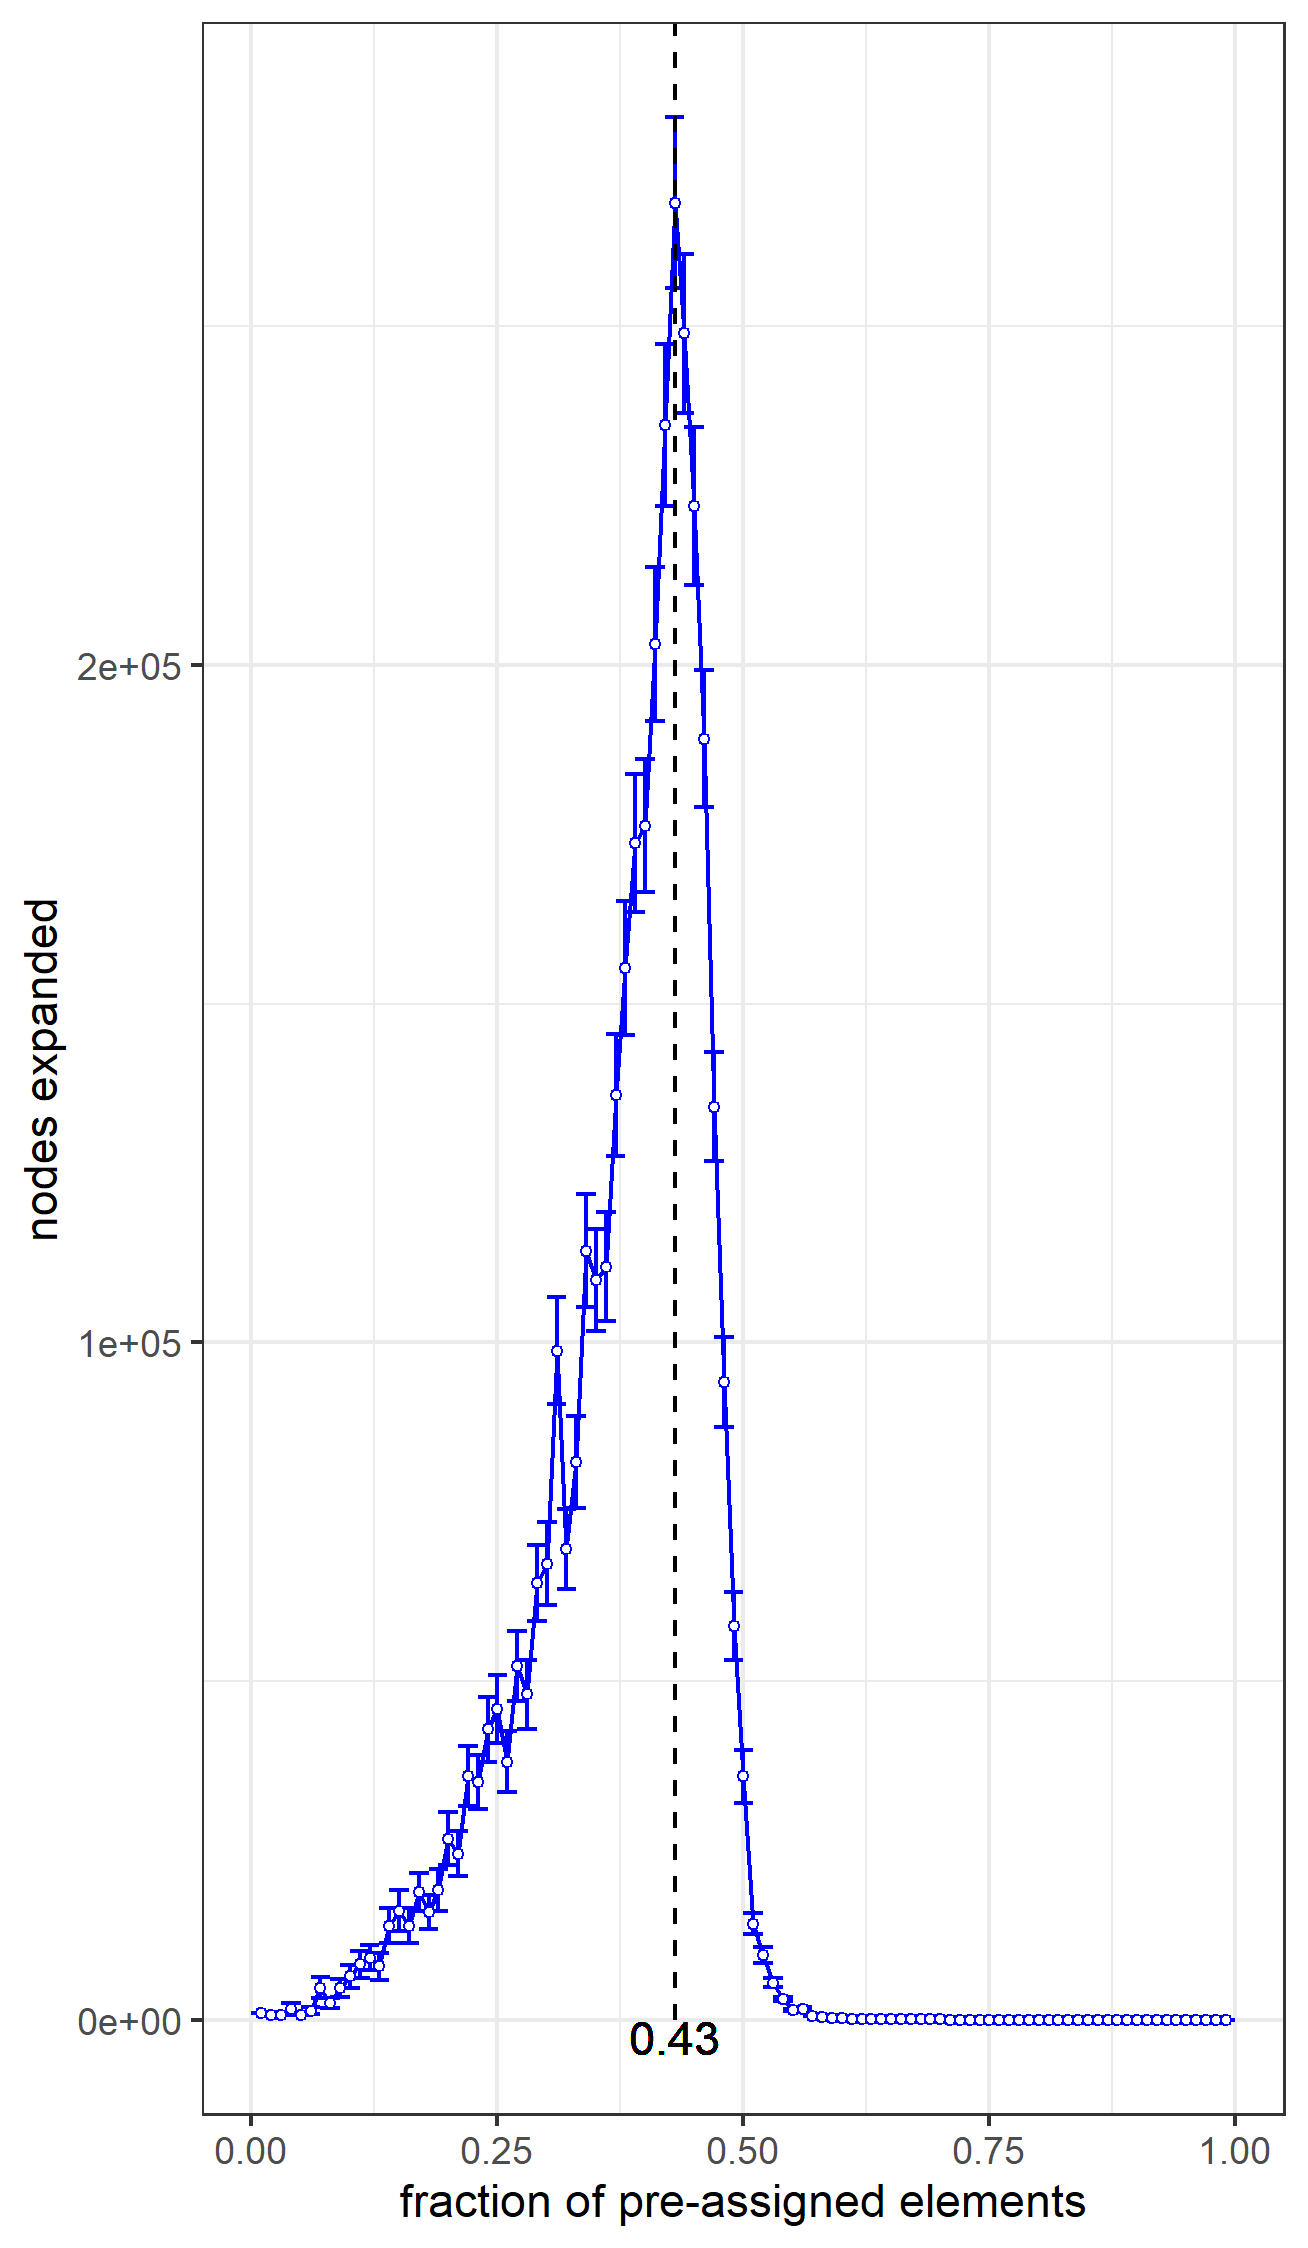
\includegraphics[width=0.4\textwidth]{img/nodes.png}
		\caption{Resultado de los nodos recorridos.}
		\label{fig:nodos}
	\end{figure}
	
	\begin{figure}[H]
		\centering
		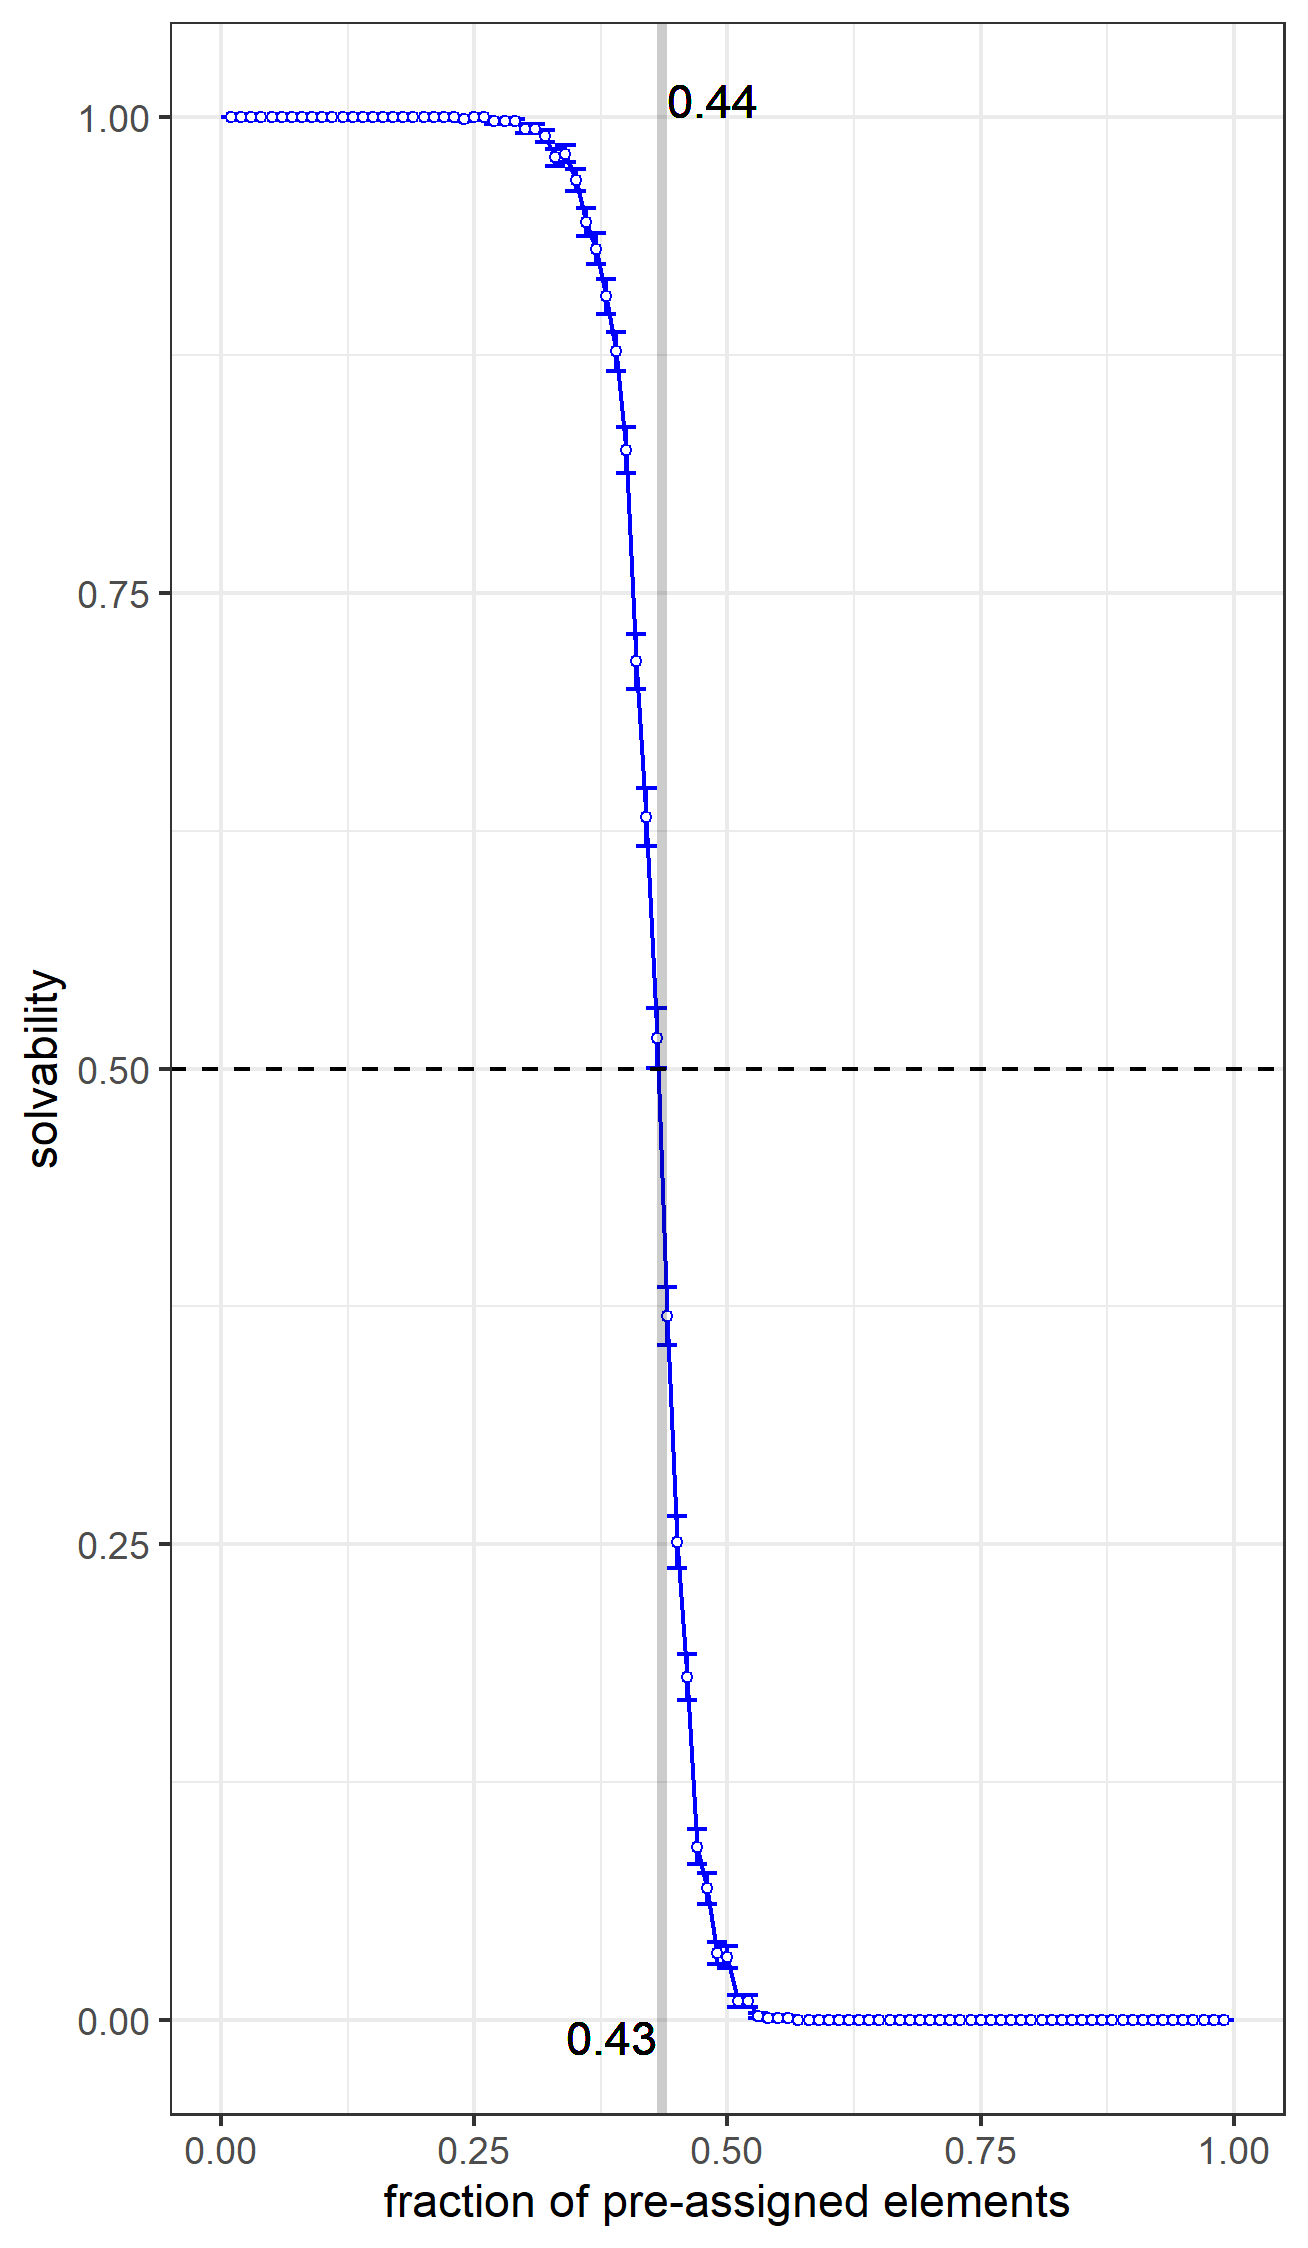
\includegraphics[width=0.4\textwidth]{img/solvability.png}
		\caption{Resultado de la solvencia del problema.}
		\label{fig:solvencia}
	\end{figure}
\end{multicols}

\end{document}
